\chapter{Analiza problemu}
\thispagestyle{chapterBeginStyle}
\label{rozdzial1}

Analiza problemu
---------------------------------
W tym rozdziale należy przedstawić analizę zagadnienia, które podlega informatyzacji. Należy zidenty-
fikować i opisać obiekty składowe rozważanego wycinka rzeczywistości i ich wzajemne relacje (np. użytkown-
ików systemu i ich role). Należy szczegółowo omówić procesy jakie zachodzą w systemie i które będą infor-
matyzowane, takie jak np. przepływ dokumentów. Należy sprecyzować i wypunktować założenia funkcjon-
alne i poza funkcjonalne dla projektowanego systemu. Jeśli istnieją aplikacje realizujące dowolny podzbiór
zadanych funkcjonalności realizowanego systemu należy przeprowadzić ich analizę porównawczą, wskazując na
różnice bądź innowacyjne elementy, które projektowany w pracy system informatyczny będzie zawierał. Należy
odnieść się do uwarunkowań prawnych związanych z procesami przetwarzania danych w projektowanym sys-
temie. Jeśli zachodzi konieczność, należy wprowadzić i omówić model matematyczny elementów systemu na
odpowiednim poziomie abstrakcji.
{\color{dgray}
W niniejszym rozdziale omówiono koncepcję architektury programowej systemu \ldots. W
szczególny sposób \ldots. Omówiono założenia funkcjonalne i niefunkcjonalne podsystemów \ldots. Przedstawiono
mechanizmy \ldots. Sklasyfikowano systemy ze względu na \ldots. Omówiono istniejące rozwiązania informatyczne o podobnej funkcjonalności \ldots (zobacz \cite{JCINodesChord}).

-Omowienie sposobow redundancji danych -RAID -Istniejace rozwiazania -Wybrane rozwiazania
-Problem rozbijania danych -Problem wielu replik -Problem synchronizacji -Problem obsługi pełnej funkcjon-
alności, np. softlinks
Założenia: -Rodzaj wykorzystywanego sposobu redundacji niewidoczny dla uzytkownika -Uzytkownik nie
martwi sie replikami poza wyjatkowymi sytuacjami: synchronizacja replik przy zamontowaniu, zatwierdzenie
korekty
}

\begin{itemize}
    \item Obsługa kilku różnych rozwiązań redundancji
    \item Obsługa wielu replik dla większego bezpieczeństwa danych 
    \item Wybór najodpowiedniejszej repliki do odczytu danych
    \item Synchronizacja istniejących danych pomiędzy replikami przy zamontowaniu systemu plików
	\item Obsługa przynajmniej podstawowych zachowań systemu plików:
		\begin{itemize}
			\item Czytanie oraz pisanie do plików
			\item Tworzenie oraz usuwanie plików
		\end{itemize}
	\item Detekcja błędów:
		\begin{itemize}
			\item Sprawdzanie, czy pliki, na których dokonywane są operacje, nie są uszkodzone
			\item Sprawdzanie synchronizacji danych między replikami
		\end{itemize}
	\item Korekcja błędów:
		\begin{itemize}
			\item Zastosowanie kodów korekcyjnych
			\item Całkowite zastępowanie uszkodzonych danych replikami
		\end{itemize}
    \item Wygoda uzytkowania
\end{itemize}

\section {Redundancja danych}
Redundancja danych stanowi najwazniejsze zagadnienie rozwazanej pracy. Zaproponowano kilka roznych rozwiazan, aby przedstawic pozadany zakres mozliwosci systemu. Rozwiazania oparte sa na macierzy RAID ze wzgledu na ich skutecznosc oraz mozliwosc tworzenia kombinacji standardowych poziomow.

wspomniec o tym ze pomimo nazwy replika mozna miec np jedna i to ma zerowa redundancje ew korekte
\subsection {RAID}
Redundant Array of Independent Disks to metoda wirtualizacji przechowywania danych. Wykorzystuje wiele dyskow i laczy je w logiczne jednostki pamieci. RAID jest stosowane do redundancji danych oraz lepszej wydajnosci, jednak w niniejszej pracy wydajnosc systemu nie bedzie rozwazana.  
RAID jest zbiorem schematow rozwiazan, ktore nazywane sa poziomami. Na potrzeby pracy przedstawione zostana wybrane poziomy, ktore wprowadzaja rozne metody redundancji.
\subsubsection{Poziom 0}
\begin{figure}[h!]
        \centering
        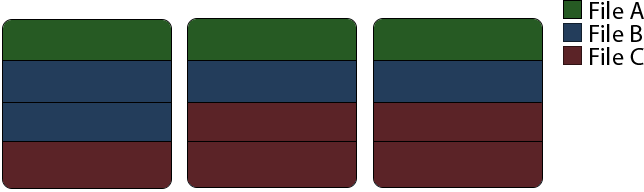
\includegraphics{raid-0.png}
        \caption{RAID-0 z trzema dyskami}
        \label{fig:raid0}
\end{figure}
\subsubsection{Poziom 1}
\begin{figure}[h!]
        \centering
        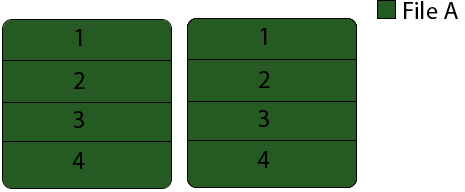
\includegraphics{raid-1.png}
        \caption{RAID-1 z dwoma dyskami}
        \label{fig:raid1}
\end{figure}
\subsubsection{Poziom 2}
dupa
\begin{figure}[h!]
        \centering
        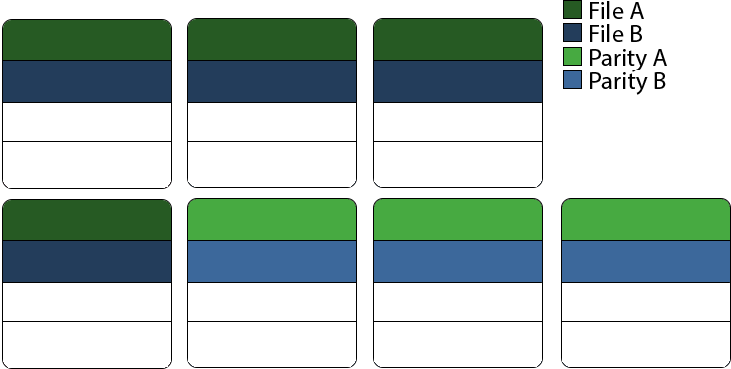
\includegraphics{raid-2.png}
        \caption{RAID-2 na siedmiu dyskach}
        \label{fig:raid2}
\end{figure}
\subsubsection{Poziom 4}
dupa
\begin{figure}[h!]
        \centering
        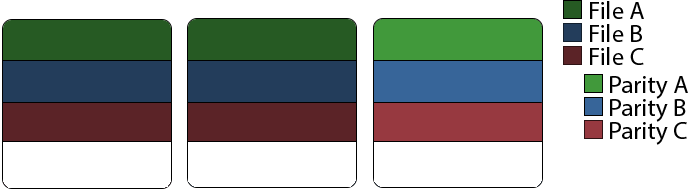
\includegraphics{raid-4.png}
        \caption{RAID-4 na trzech dyskach}
        \label{fig:raid4}
\end{figure}
\subsubsection{Poziom 5}
dupa
\begin{figure}[h!]
        \centering
        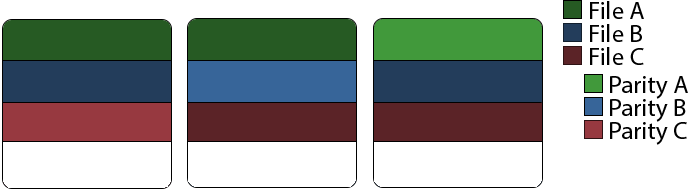
\includegraphics{raid-5.png}
        \caption{RAID-5 na trzech dyskach}
        \label{fig:raid5}
\end{figure}
\subsubsection{Poziom 6}
dupa

\newpage
\subsection{Standardowe repliki systemu}
Repliki zostaly zaprojektowane na podstawie poziomow RAID. Roznia sie miedzy soba sposobem wprowadzenia redundancji danych oraz mozliwym zastosowaniem. Ponizej opisano proponowane rodzaje replik oraz rozwazono ich mocne i slabe strony. Wszystkie rodzaje mozna podzielic na dwie kategorie:
\begin{itemize}
    \item Replika standardowa - Dokonuje detekcji bledow w plikach, jednak w przypadku wykrycia takiego bledu lub desynchronizacji z innymi replikami, nie jest w stanie dokonac korekty bledow bez dodatkowych replik
    \item Replika korekcyjna - Dokonuje zarowno detekcji, jak i korekcji znalezionych bledow. Jesli korekta znalezionych bledow jest niemozliwa, zachowuje sie podobnie do repliki bez korekty - desynchronizacja moze zostac naprawiona wylacznia z dodatkowymi replikami
\end{itemize}
Repliki korekcyjne dodają funkcjonalność do standardowej, dlatego zostały omówione w późniejszej sekcji pracy. 

\subsubsection{Repliki Lustrzane (MR)}
Oparte na schemacie RAID-1 repliki tego typu stanowią lustrzane odbicie danych. Funkcjonalność takie systemu jest równa systemowi nadrzędnemu. 
\begin{itemize}
        \item Naprawia błędy innych replik kopiując całe pliki
        \item Wszystkie dane zamontowane w jednym miejscu. W przypadku, kiedy jeden dysk zostanie uszkodzony, dane zostają utracone.
\end{itemize}

\begin{figure}[h!]
        \centering
        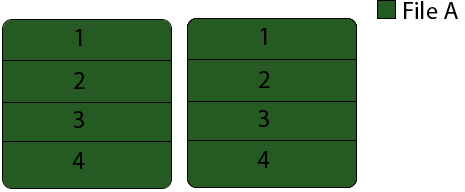
\includegraphics{raid-1.png}
        \caption{Dwie repliki blokowe}
        \label{fig:raid1}
\end{figure}

Standardowe MR nie są w stanie naprawić uszkodzonych plików. Jedynym rozwiązaniem jest zastąpić uszkodzone pliki w całości danymi z innej repliki. Niestandardowymi MR nazywa się repliki lustrzane z korektą błędów.
\subsubsection{Repliki Blokowe (BR)}
W replikach tego typu pliki są rozkładane na części i zapisywane w kolejnych katalogach będących odpowiednikiem dysków poziomu RAID-0. Tak samo katalogi mogą być rozmieszczone na różnych urządzeniach przechowujących. Każdy z katalogów może również być repliką. Jedna część pliku nazywana jest dalej blokiem.
Rozkład danych jest możliwy na dwa sposoby:
\begin{itemize}
    \item Pliki podzielone na stałą ilość bloków o zmiennych wielkościach. 

            Zmiana wielkości pliku może powodować zmianę rozmiaru wszystkich bloków danego pliku dla wyrównania wielkości, lub jedynie tego bloku, do którego dane zostają dopisane. W takim wypadku bloki nie są jednakowych rozmiarów.
            \begin{figure}[h!]
                    \centering
                    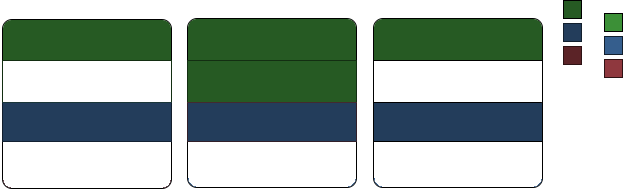
\includegraphics{BR-1.png}
                    \caption{Podział pliku na trzy nierówne bloki }
                    \label{fig:br1}
            \end{figure}
    \item Pliki podzielone na zmienną ilość części o ograniczonych wielkościach

            Określony jest maksymalny dozwolony rozmiar dla pojedynczego bloku. Przy przekroczeniu rozmiaru bloku, system tworzy kolejny w następnym katalogu dopóki jest miejsce. 
            \begin{figure}[h!]
                    \centering
                    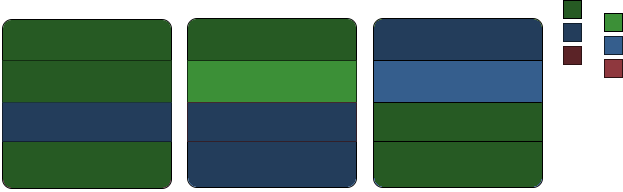
\includegraphics{BR-2.png}
                    \caption{Podzial pliku na wiele bloków ograniczonego rozmiaru}
                    \label{fig:br1}
            \end{figure}
 
\end{itemize}
Standardowe BR nie są w stanie naprawić uszkodzonych plików, jednak taki podział danych wpłynie korzystnie na repliki korekcyjne i jest szczególnie przydatny dla wielu dysków.
\begin{itemize}
    \item Naprawia błędy innych replik kopiując jedynie częściowe pliki, jeśli to możliwe.
    \item Dane mogą zostać zamontowane w wielu miejscach. W przypadku uszkodzenia jednego dysku, reszta danych jest nadal dostępna.
\end{itemize}

\subsection{Podzial replik na warstwy}

\section {Detekcja błędów}
    Wykrywanie bledow wspomaga replikowanie oraz korekte, informujac system o niezawodnosci danych. Wszystkie techniki detekcji bledow dodaja kolejne dane do zapisu, tym samym zwiekszajac redundancje w systemie. Kazda metoda ma kilka roznych rozkladow danych wynikajacych ze struktury replik, jednak w niniejszym rozdziale omowione zostana ogolne modele tych technik. Niektore metody detekcji przy odpowiednich warunkach moga od razu dokonywac korekty wykrytych bledow, co zostalo dokladniej opisane w kolejnym punkcie.

    Poprawna detekcja bledow moze umozliwic naprawe uszkodzonych plikow bez wiedzy uzytkownika.
\section {Korekcja błędów}

\subsection{Kod Hamminga}
\subsection{Parzystość}
\subsection{Repliki korekcyjne}

Dodanie metod korekcji błędów w replikach BR umożliwi odzyskiwanie całych bloków. W przypadku uszkodzonego dysku, repliki BR mogą być w stanie zmienić lokalizację odzyskanego bloku lub zmienić sposób, w jaki dzielą dane. To znaczy, że jeśli replika blokowa działa na n dyskach, działa również po awarii na n-1 dyskach dla n < 1.

\section {Synchronizacja replik}

\section {Dzialanie systemu plikow}

\section {Wygoda uzytkowania}
